% 12pt .6pt grayscale fragment; standalone tikz; no document env
\usetikzlibrary{arrows.meta,calc}
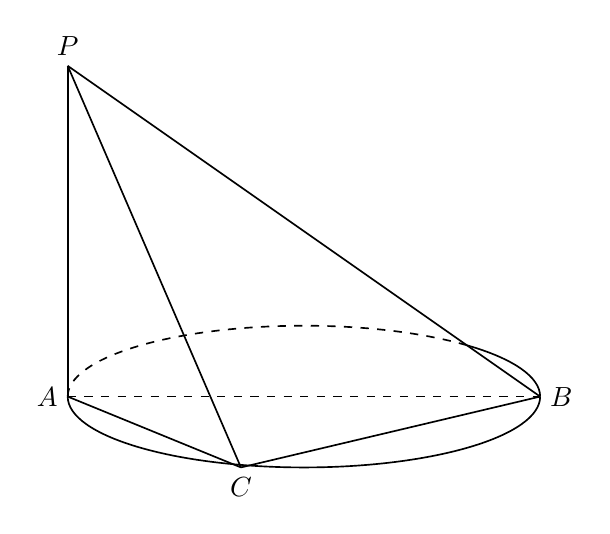
\begin{tikzpicture}[line width=0.6pt,>=Stealth,font=\normalsize]
\coordinate (A) at (0,0);
\coordinate (B) at (6,0);
\coordinate (C) at (2.2,-0.9);
\coordinate (P) at (0,4.2);
\draw (B) arc (0:46.3971810273:3 and .9);
\draw[dashed] ({3+3*cos(46.3971810273)},{.9*sin(46.3971810273)}) arc (46.3971810273:180:3 and .9);
\draw (3,0) ++(-3,0) arc (180:360:3cm and 0.9cm);
\draw (P)--(A);
\draw[dashed] (A)--(B);
\draw (P)--(B);
\draw (P)--(C);
\draw (A)--(C);
\draw (B)--(C);
\node[above] at (P) {$P$};
\node[left] at (A) {$A$};
\node[right] at (B) {$B$};
\node[below] at (C) {$C$};
\end{tikzpicture}
